\documentclass[../main.tex]{subfiles}
\graphicspath{{\subfix{../figures/}}}
%
\begin{document}
%
\section{静态建模}
该系统中出现的实体对象有用餐人员、餐桌、菜品分类、菜品、点餐记录(订单)、
配餐工作人员、一体机等信息实体.

根据常识和需求的描述,我们可以识别出以下类:
\begin{itemize}
  \item 用餐人员(Customer):负责在食堂APP上进行点餐和结算操作。具有账号注册、浏览菜品、选择菜品、调整数量、终止点餐、在线充值等功能。
  \item 菜品分类(Category):表示食堂菜品的分类。
  \item 菜品(Dish):表示具体的菜品,包含名称、配料和价格等信息。
  \item 点餐记录(Order):表示用餐人员的点餐记录,包括餐位号、菜品及其份数。
  \item 配餐工作人员(Worker):负责根据点餐结果进行配餐的工作人员。拥有一台带有触摸屏和打印机的一体机,接收分配给他的配餐任务。
\end{itemize}
%
于是我们可以得到以下的类图:
\begin{figure}[H]
  \begin{center}
    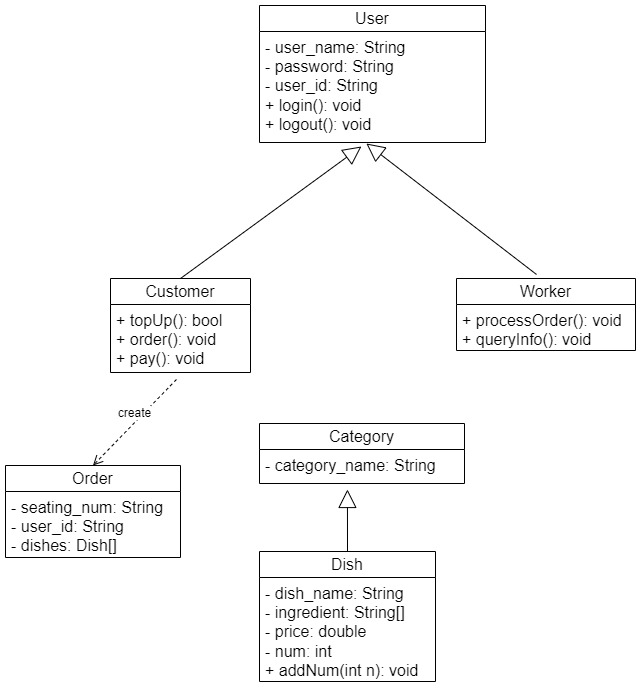
\includegraphics[width=0.65\textwidth]{类图.jpg}
  \end{center}
  \caption{智慧食堂系统类图}
\end{figure}
%
\end{document}
